This chapter provides an overview of \acp{MAS}, as a mean to engineer intelligent applications.
%
\acp{MAS} are a broad research area at the intersection between \ac{AI} and software engineering.
%
Autonomous agents are used as the main abstraction to model and implement complex software systems. The behavior of such agents can be either programmed, learned or, more recently, generated through the use of \ac{GenAI} techniques. 

In this thesis, we mainly consider programmed agents, as we are interested in using agents to encapsulate business logic that can automate processes and activities in the context of \ac{DT}-based systems. 
%
Accordingly, the chapter introduces the research area which follows under the broad umbrella of \ac{AOSE} and more specifically \ac{AOP} as a paradigm to engineer and program \acp{MAS}. 
%
We specifically focus on \ac{BDI} agents, as they are amongst the most widely adopted agent model for programmed agents, capable of encoding domain and procedural knowledge through the cognitive abstractions they provide, thus making \ac{BDI} agents excellent candidates for reliable and explainable intelligent applications. 

%=======================================================
\section{History and Definitions}
%=======================================================

In order to understand the concept of \acp{MAS}, it is important to first understand what an \emph{agent} is.
%
Despite the term being widely used in different contexts~\cite{wooldridge1995ker} with different interpretations, a commonly accepted definition is the following:

\begin{quote}
    An agent is a computer system that is situated in some environment,
    and that is capable of autonomous action in this environment in order
    to meet its design objectives~\cite{2009wooldridge}.
\end{quote}

The definition highlights the key characteristics of an agent. 
%
Namely, an agent is \emph{situated} in an environment which can be either physical (e.g., for a robotic system) or virtual (e.g., for a fully software agent).
%
The environment provides the agent with an external context that can be perceived, influencing the behavior of the agent, and affected by the agent actions to reach its objectives.
%
\Cref{fig:agent-environment} shows the relationship between an agent and its environment. The agent receives \emph{percepts} from the environment through its sensors, and performs actions upon the environment through its \emph{effectors}.
%
The agent is also \emph{autonomous}, meaning that it can operate without direct intervention from humans or other systems, and has control over its actions and internal state.
%
Finally, the agent is \emph{goal-oriented}, as it is designed to achieve specific objectives, which can be explicitly defined or learned over time.

\begin{figure}[t]
    \centering
    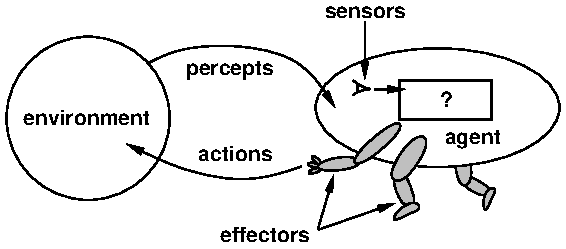
\includegraphics[width=0.8\textwidth]{figures/agent-environment-original.pdf}
    \caption{Classic schematic representation of an agent and its interaction with the environment, from \cite{1995russell-norvig}.}
    \label{fig:agent-environment}
\end{figure}

It is possible to distinguish between a \emph{weak} and \emph{strong} notion of agency~\cite{wooldridge1995ker}.
%
The weak notion of agency refers to systems that exhibit some characteristics of agents, namely autonomy, reactivity, pro-activeness, and social ability. 
%
This kind of agents are usually employed to model concurrent and distributed systems. 
%
The strong notion of agency, instead, derives from research on \ac{AI} and envisions agents as \emph{intelligent} entities, modeled using \emph{mentalistic} notions~\cite{Shoham_1993} to mimic human cognitive capabilities. 

The definitions of \emph{agent} focus on the properties of an agent and its behavior, leaving implementation details open. 
%
This has led to the development of different agent architectures to implement agents in software systems. 
%
The taxonomy of agent models proposed by Russell and Norvig~\cite{1995russell-norvig} distinguishes between increasingly complex agent models: 
\begin{description}
    \item[Simple Reflex Agents] operate on a set of predefined trigger-action rules and to respond to stimuli from the environment.
    \item[Model-Based Reflex Agents] keep an internal model of the environment, updating it over time, and allowing them to make decisions based on both current perceptions and past experiences.
    \item[Goal-Based Agents] are designed to achieve specific goals. They can evaluate different actions not only based on the model of the environment, but also on the potential of achieving their goal, allowing for more flexible and adaptive behavior.
    \item[Utility-Based Agents] not only aim to achieve goals but also consider the desirability of different outcomes. They use a utility function to evaluate the potential benefits of various actions, enabling them to make decisions that maximize overall satisfaction.
    \item[Learning Agents] can improve their performance over time through learning from experiences. They can adapt to changing environments and optimize their behavior based on feedback, making them more robust and effective in dynamic settings.
\end{description}

Implementing an agent essentially boils down to specify its behavior in response to its perceptions of the environment, with different degrees of complexity. 
%
How this is achieved depends on the agent architecture and model adopted, but we can generally  distinguish two main categories: \emph{programmed} or \emph{learning} agents, depending on whether their behavior is explicitly defined by a developer or learned from data and experience. 
%
Although the boundary between the two categories is not always clear-cut, as learning techniques can be used to complement programmed behavior~\cite{Bordini_El_Fallah_Seghrouchni_Hindriks_Logan_Ricci_2020,Bosello_Ricci_2020}, they provide a useful distinction to understand the different approaches to implement agents.
%
The involved techniques are, in fact, quite different.
%
While programmed agents rely on either pre-specified behavior (e.g., rules, decision trees) or assemble it dynamically through planning algorithms~\cite{Ghallab_Nau_Traverso_2004},
learning agents require a different a training phase where machine learning techniques are employed to learn patterns and behaviors from data.
%
The most common learning technique for agents is \ac{RL}, where agents learn to make decisions by interacting with the environment and receiving feedback in the form or reward or punishment based on their actions, thus learning a \emph{policy} to maximize the cumulative reward over time~\cite{Sutton_Barto_1998}.

Recently, the advent of \ac{GenAI} techniques, has brought new opportunities to implement agents. \emph{Agentic \ac{AI}}~\cite{Acharya_Kuppan_Divya_2025} refers to the use of \ac{GenAI} models, such as \acp{LLM}, to create agents that can perform tasks autonomously by generating responses and actions based on natural language prompts.
%
Agents based on these techniques can be seen as a third category of agents, where the behavior is neither explicitly programmed nor learned from experiences, but rather synthesized on-the-fly by the generative model based on the context and instructions provided.

Having defined what an \emph{agent} is, a \emph{\acl{MAS}} is, finally, a system composed of multiple interacting agents, which can be either cooperative or competitive, working together to achieve individual or shared goals~\cite{2009wooldridge}.
%
The interaction between agents can be direct, through agent-to-agent communication~\cite{Kone_Shimazu_Nakajima_2000}, or indirect, through the manipulation of the shared environment they operate in~\cite{Weyns_Omicini_Odell_2007}.

\ac{MAS} are particularly useful for modeling and solving complex problems that are difficult to tackle with traditional approaches.
%
The behavior of a \ac{MAS} emerges from the interactions of its agents, allowing to break down complexity into manageable components whose behavior can be defined independently.
%
In the case of learning agents, \ac{MARL} techniques tackle the problem of training multiple agents at the same time, considering the interactions and dependencies between them~\cite{Albrecht_Christianos_Schäfer_2024}.


Due to their versatility, \ac{MAS} have been adopted in various domains, including robotics~\cite{Vicente-Diaz_2012}, (social) simulation~\cite{Uhrmacher_Weyns_2018,Davidsson_2001}, and distributed control systems for smart grids~\cite{Merabet_Essaaidi_Talei_Abid_Khalil_Madkour_Benhaddou_2014}, \ac{IoT}~\cite{Singh_Chopra_2017}, or traffic management~\cite{Torabi_Wenkstern_Saylor_2020}.

Considering this very broad landscape, in this thesis, when referencing to agents,  we refer to \emph{programmed} agents and specifically on \ac{BDI} agents as an example of systems with a \emph{strong} notion of agency.
%
The goal is to leverage the cognitive abstractions provided by \ac{BDI} agents to model and implement predictable, reliable and explainable intelligent behavior in \ac{DT}-based systems, encoding domain knowledge and business logic in the agents' mental state and plans.

%=======================================================
\section{\acl{AOSE}}
\label{sec:back:mas:aose}
%=======================================================

The engineering of \acp{MAS} is a complex task, as it involves designing each individual agent and their interactions with each other and the environment.
%
Hence, the research area of \ac{AOSE} has been developed as a sub-field of software engineering, focusing on the engineering of distributed systems using agent-oriented abstractions~\cite{Jennings_1999,Wooldridgey_Ciancarini_2001}.

A big effort in \ac{AOSE} has been devoted to the definition of methodologies to guide the analysis, design and implementation of distributed systems through the agent abstraction~\cite{Wooldridgey_Ciancarini_2001}.
%
Notable examples of such methodologies include Gaia~\cite{Wooldridge_Jennings_Kinny_2000}, Tropos~\cite{Giunchiglia_Mylopoulos_Perini_2002}, Prometheus~\cite{Padgham_Winikoff_2002}, INGENIAS~\cite{Pavón_Gómez-Sanz_2003}, and PASSI~\cite{Cossentino_2005}.
%
Nevertheless,
despite the abundance of methodologies born within the \ac{AOSE} community, their adoption in mainstream software engineering has been limited~\cite{Gómez-Sanz_Fuentes-Fernández_2015}.
%
Most methodologies focused only on requirement analysis, modeling agent interactions, roles, and behaviors and some provide supporting tools in the form of diagrams and code generation plugins~\cite{Bergenti_Gleizes_Zambonelli_2006,Gómez-Sanz_Fuentes-Fernández_2015}. 
%
The developed system was then free to be implemented using any general-purpose programming language, without necessarily having a direct mapping between the agent-oriented design abstractions and the implementation constructs. 

Complementing the high-level design-oriented efforts of \ac{AOSE} methodologies, \ac{AOP} has been proposed envisioning agents not only as a design abstraction, but also as a programming concept to practically implement software systems~\cite{Shoham_1993}.
%
In \ac{AOP} agents are considered the fundamental building blocks of a software systems (just like objects are in \ac{OOP}, and functions are in \ac{FP}), and the development of a software system involves defining the agents, their behaviors, and their interactions.
%
\ac{AOP} specifically targeted the \emph{strong} notion of agency, hence characterizing the state of agents using mentalistic notions such as beliefs. Furthermore, agents in \ac{AOP} interact by means of messages following an \ac{ACL}
based on speech act theory~\cite{Austin_1975}.
%
The intended purpose of \ac{AOP} is to encode complex behavior in a natural and intuitive language, that supports high-level abstractions to model the decision-making process of agents, as well as their interactions. 

The work on \ac{AOP} has led to development frameworks and programming languages specifically designed specifying agent behavior, providing tools and libraries to facilitate the implementation of \ac{MAS}~\cite{Cardoso_Ferrando_2021}.

When scaling the complexity from single agents to a \ac{MAS}, it has been recognized that also other programming abstractions are needed other than agents alone (\Cref{fig:mas-dimensions-overview}). 
%
These \emph{dimensions} of \ac{MAS} programming, 
other than the aforementioned \emph{agent} dimension,
include the \emph{environment} dimension~\cite{Weyns_Omicini_Odell_2007} which focuses on the design of the shared environment in which the agents operate,
the \emph{interaction} dimension~\cite{Huhns_2001} which focuses on the communication and coordination mechanisms between agents,
and the \emph{organization} dimension~\cite{Boissier_Hübner_Sichman_2007} which focuses on the structure and roles of agents within the \ac{MAS}.
%
Focusing on different dimensions, allows to address the same problem in different ways, as each dimension provides different abstractions and mechanisms to model and implement the behavior of a \ac{MAS}~\cite{Boissier_Bordini_Hübner_Ricci_2019}.

\begin{figure}[t]
    \centering
    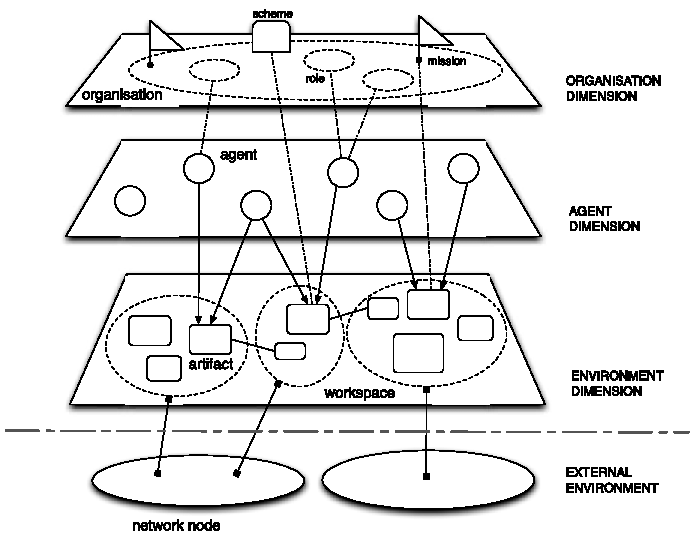
\includegraphics[width=0.9\textwidth]{figures/mas-dimensions-overview.pdf}
    \caption{High-level overview of the main programming dimensions of a \ac{MAS}, the \emph{interaction} dimension, not shown, focuses on interaction between agents, from \cite{Boissier_Bordini_Hübner_Ricci_Santi_2013}.}
    \label{fig:mas-dimensions-overview}
\end{figure}


The environment programming dimension has been introduced to recognize the environment as a first-class abstraction in \ac{MAS} programming~\cite{Weyns_Omicini_Odell_2007}.
%
In this perspective, the environment is not just a passive context, but an active component that can influence and be influenced by agents.
%
Namely, the environment can serve three major roles in supporting the activity of a \ac{MAS} at different levels: 
\begin{itemize}
    \item at a \emph{Basic Level} the environment provides access to the deployment context of the agent, allowing it to interact with external resources either them being physical (e.g., sensors, actuators) or virtual (e.g., databases, web services);
    \item at an \emph{Abstraction Level}, the environment provides a higher-level representation of the context in which agents operate bridging the gap between the low-level details and the agents' behavior;
    \item at a \emph{Interaction-mediation Level}, the environment facilitates the communication and coordination between agents, regulating access to shared resources and hence becoming an active entity in the \ac{MAS}.
\end{itemize}


Elaborating on this perspective, the \emph{Agents and Artifacts (A\&A)} metamodel, proposes to model the environment as a collection of \emph{artifacts} shared amongst agents~\cite{Omicini_Ricci_Viroli_2008}.
%
Artifacts are defined as computational entities that encapsulate both state and behavior, providing a means for agents to interact with the environment in a structured way.
%
This approach allows for a more flexible and dynamic modeling of the environment, introducing a further \emph{reflection level} where artifacts can be created, modified, and destroyed at runtime by the agent themselves, reflecting the changing needs and goals of the agents~\cite{Ricci_Omicini_Viroli_Gardelli_Oliva_2007}.

The organization programming dimension~\cite{Boissier_Hübner_Sichman_2007} focuses on the structure and roles of agent societies within a \ac{MAS}. 
%
\ac{MAS} organizations shift the focus from individual agents to the collective behavior of groups of agents~\cite{Ferber_Gutknecht_Michel_2004}.
%
Organization programming targets those kinds of \ac{MAS} where the strcture and roles within an organization are explicitly defined and managed in a top-down fashion, as opposed to emergent organizations where the structure arises from the interactions of individual agents in a bottom-up fashion~\cite{Boissier_Hübner_Sichman_2007}.

\begin{figure}[t]
    \centering
    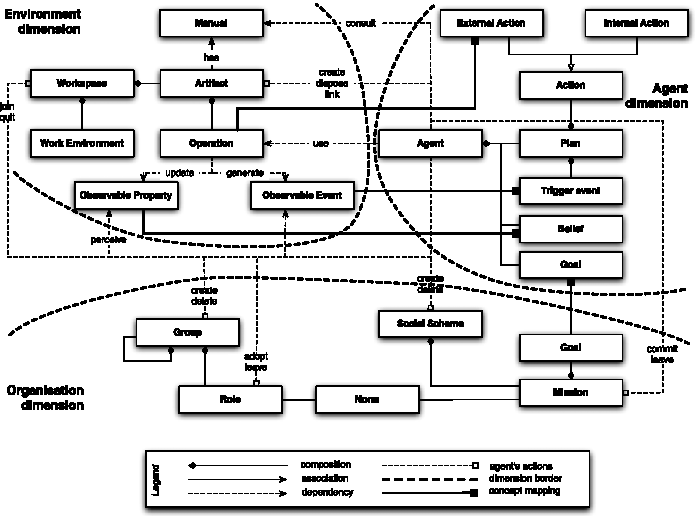
\includegraphics[width=\textwidth]{figures/mas-dimensions-schema.pdf}
    \caption{Schematic representation of the main abstractions of \ac{MAOP} and their relationships, from \cite{Boissier_Bordini_Hübner_Ricci_Santi_2013}.}
    \label{fig:mas-dimensions-schema}
\end{figure}

The proposal of \ac{MAOP} evolves \ac{AOP} to consider all the different dimensions of \ac{MAS} programming in a unified framework~\cite{Boissier_Bordini_Hübner_Ricci_Santi_2013,Boissier_Bordini_Hubner_Ricci_2020}.
%
The paradigm has been supported by the development of the \jacamo{}~\cite{Boissier_Bordini_Hubner_Ricci_2020} framework which integrates three main components:
\begin{itemize}
    \item \textbf{\jason{}}: a Java-based interpreter of \agentspeak{}~\cite{raoagentspeak} for programming and executing \ac{BDI} agents~\cite{Bordini_Hübner_Wooldridge_2007};
    \item \textbf{\cartago{}}: a framework to model and implement the environment as a set of artifacts that agents can use to perceive and act upon the environment~\cite{Ricci_Piunti_Viroli_Omicini_2009};
    \item \textbf{\moise{}}: a framework to define and manage the organization of agents in terms of roles, groups, and missions~\cite{Boissier_Hübner_Sichman_2007}.
\end{itemize}

\ac{MAOP} and the \jacamo{} framework have been widely influential in the \ac{AOSE} community, providing an integrated foundation for the engineering of complex \acp{MAS}~\cite{Boissier_Bordini_Hubner_Ricci_2020}.
%
\Cref{fig:mas-dimensions-schema} provides a representation of how the different programming dimensions of a \ac{MAS} are integrated in the \ac{MAOP} paradigm, showing the main abstractions and their interrelations.

In this thesis, when we discuss the engineering of \ac{MAS} we follow a \ac{MAOP}-inspired approach, focusing on the agent and the environment dimensions (and the A\&A metamodel in particular), as they are the most relevant for the integration of \acp{MAS} with \ac{DT}-based systems.
%
Although the organization dimension is also relevant, we do not specifically address it in this thesis, as we focus on relatively small-scale \acp{MAS} where the organization is implicit.

%=======================================================
\section{\acl{BDI} Agents}
%=======================================================
The \ac{BDI} model originated from the philosophical theory of human practical reasoning developed by Michael Bratman~\cite{Bratman1987-BRAIPA}.
%
The theory focused on the notion of \emph{intention} (i.e., the commitment to carrying out a plan of action), to describe future-directed decision-making, explaining how humans decide what to do
when they have multiple desires and goals to achieve.

The model influenced the development of computational agents~\cite{rao1991modeling}, 
leading to agent architectures such as the \ac{PRS}~\cite{Georgeff_Lansky_1986},
which provides a framework for implementing \ac{BDI} agents in software systems.
%
Computational \ac{BDI} agents are characterized by the following main abstractions:
%
\begin{description}
    \item[Beliefs:] a set of facts and rules representing an agent's memory, collecting knowledge about its perception of the world, itself, and other agents;

    \item[Desires:] a set of goals, representing (possibly partial) descriptions of desirable states of the world
    the agent is willing to achieve, test, or maintain;

    \item[Intentions:] a set of tasks the agent is currently committed to, in order to satisfy some of its desires;

    \item[Plans:] a set of \emph{recipes} representing the agent's procedural memory,
    hence encoding the know-how about achieving a given intention under certain conditions.
\end{description}


\begin{figure}[t]
    \centering
    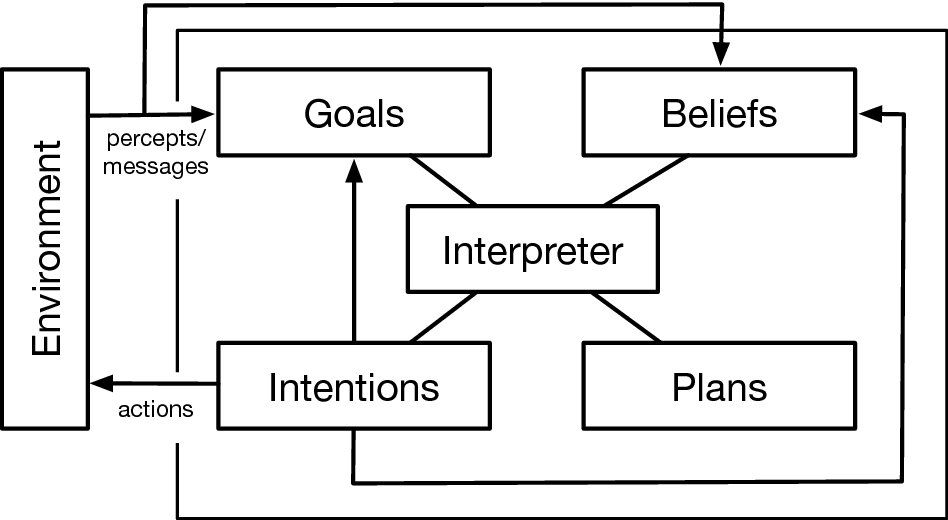
\includegraphics[width=0.9\textwidth]{figures/bdi-agent-schema.png}
    \caption{Schematic, high-level representation of a \ac{BDI} agent, from \cite{Bordini_El_Fallah_Seghrouchni_Hindriks_Logan_Ricci_2020}.}
    \label{fig:bdi-model}
\end{figure}


\Cref{fig:bdi-model} shows how these abstractions relate to each other in a schematic representation of a \ac{BDI} agent.
%
The agent acquires percepts and receives messages from other agents through the environment. This can lead to an update of the agent's beliefs or goals.
%
Based on its beliefs and goals, the agent deliberates on intentions to commit to, and selects plans to achieve them. 
%
Finally, pursuing an intention, through the execution of the selected plans may lead to actions that affect the environment. 
%
In the figure, a central \emph{interpreter} of the agent program is shown. 
%
This component is responsible for managing the agent's execution, often referred to as the \emph{reasoning cycle} of the agent.

\ac{BDI} agents continuously cycle through a reasoning process which involves three main phases:
\begin{enumerate}
    \item \emph{Perception:} the agent perceives its environment through its sensors, updating its beliefs accordingly;

    \item \emph{Deliberation:} the agent deliberates on its desires and intentions,
    possibly revising them in light of the updated beliefs;

    \item \emph{Action:} the agent selects and executes one or more plans to carry on its current intentions,
    possibly affecting the environment through its actuators.
\end{enumerate}

Through this mechanism, agents continuously adapt their behavior to the changing environment, acquire new beliefs that may influence their future behavior, and pursue their goals by executing plans.

Programming a \ac{BDI} agent involves defining its initial beliefs, goals, and a set of plans that support the agent in achieving its goals under different conditions. 
%
The \ac{BDI} model has been initially formalized with a logical language, \agentspeak{}~\cite{raoagentspeak} which later has inspired several agent programming languages. 
%
Amongst them \jason{}~\cite{Bordini_Hübner_Wooldridge_2007} is a Java-based interpreter for an extended version of \agentspeak{}, keeping the original syntax and semantics.

Custom \ac{BDI} agent programming languages, support developers in implementing \ac{BDI} agents by providing high-level abstractions and constructs that facilitate the definition of beliefs, goals and plans. 
%
This has the benefit of allowing developers to focus on the agent's behavior, rather than low-level implementation details. 

% \todo{reference other languages}

% \todo{explain why we consider agentspeak and jason here}

\todo{description of agentspeak?}

\todo{code examples??}

%=======================================================
\section{Web-based and Hypermedia \acs{MAS}}
\label{sec:back:mas:web}
%=======================================================

When introducing the Semantic Web (see \Cref{chap:back:Web}), Berners-Lee et al.\ envisioned a future where software agents would roam the Web, accessing and processing information on behalf of users~\cite{berners2023semantic,Hendler_2001}.

The relationship between \acp{MAS} and the Web has been widely explored especially in the context of service-oriented computing~\cite{Singh2004}.
%
Agents were seen as a natural fit to automate the composition of Web services due to their autonomy, social ability and goal-driven behavior.
%
The Web, in turn, provides an open ever-evolving environment rich of resources and services that agents may need to discover and (learn to) use. 

Despite these early visions, the adoption of \ac{MAS} in Web-based systems has been limited.
%
The famous question ``Where are all the intelligent agents?''~\cite{Hendler_2007} provocatively highlighted the gap between the early expectations and the actual adoption of \ac{MAS} in the Web context.
%
As pointed out by the answer of McBurney and Luck~\cite{McBurney_Luck_2007}, agent-based technologies have actually been adopted ``behind the scenes'' in various application domains, including the Web, not necessarily as killer applications themselves, but as the enabling technology for the engineering of complex distributed systems.

Nevertheless, early integration of \ac{MAS} and Web services in the early 2000s were still far from the original vision of the Semantic Web.
%
They mostly focused on the composition of services through the standards available at the time (e.g., SOAP, WSDL) which relied on the Web for transport~\cite{Newcomer_2002}.
%
Similarly, on the \ac{MAS} side, the focus was primarily on the development of agent communication protocols and frameworks that could operate over the Web, with the prominent example being the \ac{FIPA} specification for communication between agents over \ac{HTTP}~\cite{fipa2002http}.

Motivated by more recent trends in Web development such as the pervasive adoption of \ac{REST}~\cite{fielding2000architectural}, and the \ac{WoT}~\cite{Guinard_Trifa_2016_book} enabling Web-based interactions with physical environments, the research area of \emph{Web-based \acp{MAS}} has regained interest in the last decade.
%
This has led to a community effort to revisit the integration between \acp{MAS} and the Web~\cite{Boissier_Ciortea_Harth_Ricci_2021,Boissier_Ciortea_Harth_Ricci_Vachtsevanou_2023} and the creation of the \emph{Autonomous Agents on the Web} \ac{W3C} Community Group\footnote{\url{https://www.w3.org/community/webagents/}} to tackle the challenges of engineering Web-based \acp{MAS}. 

\begin{figure}[t]
    \centering
    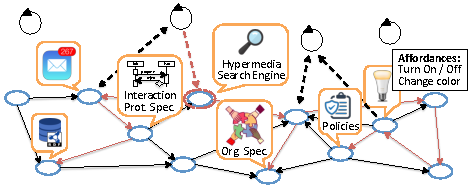
\includegraphics[width=0.9\textwidth]{figures/hmas-schema.pdf}
    \caption{Schematic representation of the concept of \acl{hMAS} showing how elements of a \ac{MAS} can be integrated and represented in a hypermedia environment for agents to discover, from \cite{Ciortea_Mayer_Gandon_Boissier_Ricci_Zimmermann_2019}.}
    \label{fig:hmas-overview}
\end{figure}

In this context, the proposal by Ciortea et al.\ envisioning \emph{\ac{hMAS}}~\cite{Ciortea_Mayer_Gandon_Boissier_Ricci_Zimmermann_2019} as a new class of Web-based \acp{MAS} is particularly relevant (\Cref{fig:hmas-overview}).
%
The proposal leverages the principles of \ac{REST}---and especially \ac{HATEOAS}---to design \acp{MAS} that are fully integrated with the Web.
%
They key, following the A\&A metamodel~\cite{Omicini_Ricci_Viroli_2008}, is to consider the Web as a shared environment where agents can operate.
%
The proposal of \ac{hMAS} is grounded on a set of principles~\cite{Ciortea_Boissier_Ricci_2019}:
\begin{itemize}
    \item \textbf{Uniform Resource Space}: every entity in the \ac{hMAS} (e.g., agents, artifacts, organizations) should be represented as resources in the hypermedia environment. 
    \item \textbf{Single Entrypoint}: given a single entrypoint to the \ac{hMAS} (e.g. a \ac{URI}), agents should be able to discover the knowledge required to participate in the \ac{MAS} by navigating the hypermedia environment. This is typically referred to the challenge of \emph{arrive and operate}.
    \item \textbf{Observability}: Resources in the \ac{hMAS} should be observable by agents, allowing them to perceive changes and react accordingly. 
\end{itemize}
%
The proposal of \ac{hMAS} has been supported by the development of the Yggdrasil framework~\cite{Ciortea_Boissier_Ricci_2019}, which provides a set of tools to develop hypermedia environments based on the A\&A metamodel, extending \cartago{} with \ac{REST}ful interfaces and hypermedia representation of artifacts. 

Developments in the area of \ac{hMAS} have shown the potential of using \ac{MAS} in dynamic Web environments, with a focus on the \ac{WoT}~\cite{Ciortea_Mayer_Michahelles_2018}.
%
In this context, the \ac{WoT} model based on \emph{affordances}~\cite{Norman_2013} is particularly interesting as it provides a natural way to model the discovery of interaction possibilities for agents in the hypermedia environment.
%
This concept has been explored proposing the addition of \emph{signifiers}~\cite{Norman_2008} as a first-class abstraction for the design of \ac{hMAS}~\cite{Vachtsevanou_Ciortea_Mayer_Lemée_2023}, hence introducing a way to guide agents in the discovery of relevant resources and interaction possibilities in order to more efficiently perceive and navigate the hypermedia environment, similarly to how humans do when browsing the Web. 

The principles and research efforts in the area of \ac{hMAS} are significant for this thesis, as they serve as a bridge between intelligent applications designed with \ac{MAS} and services and resources available on the Web, including \ac{DT}-based systems. 

%=======================================================
\section{\aclp{MAS} and \aclp{DT}}
\label{sec:back:mas:dt+mas}
%=======================================================

The relationship between \acp{MAS} and \ac{AI} tends toward the development of \acp{DT} that are more and more autonomous and capable of adapting to changing conditions in the \ac{PA} they mirror, to optimize their performance and achieve specific goals (see \Cref{sec:back:dt:ai}).
%
So-called \emph{Autonomic} or \emph{Cognitive} \acp{DT}~\cite{Minerva_Crespi_Farahbakhsh_Awan_2023} are being studied to endow \acp{DT} with self-* properties (e.g., self-optimization, self-healing, self-protection)~\cite{Kephart_Chess_2003,Feng_Gomes_Gil_Mikkelsen_Tola_Larsen_Sandberg_2022}.
%
In this context, \acp{DT} are seen as components to engineer complex autonomous \ac{CPS} through the exchange of simulation models to understand the behavior of other elements of the systems and achieve better overall coordination towards global goals~\cite{Esterle_Gomes_Frasheri_Ejersbo_Tomforde_Larsen_2021}.
%
It is hence not surprising that there is a significant overlap between the research areas of autonomous agents and \acp{MAS} and \acp{DT} and that integration between the two abstractions are being investigated~\cite{Hribernik_Cabri_Mandreoli_Mentzas_2021}.

Surveys highlight how the convergence of \ac{MAS} and \acp{DT} is growing predominantly within the manufacturing domain, with smart agriculture, smart cities and energy domains following~\cite{Pretel_Moya_Navarro_López-Jaquero_González_2024,Kalyani_Collier_2024}.
%
Healthcare is also considered as a relevant domain for \ac{MAS} and \acp{DT} combined.
Croatti et al.~\cite{Croatti_Gabellini_Montagna_Ricci_2020} discuss how \acp{DT} of relevant assets of a
healthcare organization could be used by agents to support decision-making and coordination of activities in a hospital setting.

Most work do not disclose the specific frameworks and tools used to implement \acp{MAS} and \acp{DT}, and some propose new ones, suggesting a fragmentation of uncoordinated proposals despite the substantial number of tools established within both areas~\cite{Pretel_Moya_Navarro_López-Jaquero_González_2024}.
%
This calls for more efforts in the integration of existing tools and frameworks, following established paradigms and standards, to facilitate the adoption of \acp{MAS} in \ac{DT}-based systems.

Whereas most surveyed works focus on a one-directional view of the combination of \acp{MAS} and \acp{DT}--- with agents supporting the implementation of \acp{DT}~\cite{Kalyani_Collier_2024} --- other combinations are possible. 
%
Mariani et al.\ discuss how \acp{DT} and \acp{MAS} have different characteristics and can complement each other in a synergistic way~\cite{Mariani_Picone_Ricci_2022}.
%
The integration between \ac{MAS} and \acp{DT} is envisioned through the environment dimension (\Cref{fig:mas-dt-integration}).
%
In this perspective, \acp{DT} can be seen as artifacts, digitally representing physical entities in the \ac{MAS} environment.

\begin{figure}
    \centering
    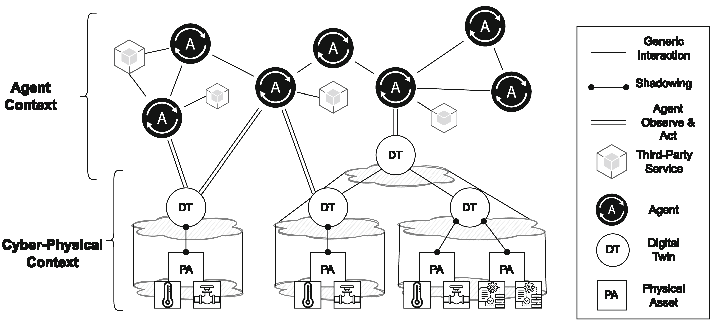
\includegraphics[width=0.9\textwidth]{figures/agent-dt-overview.pdf}
    \caption{Schematic representation of the integration between \acp{MAS} and \acp{DT} through the environment dimension, from \cite{Mariani_Picone_Ricci_2022}.}
    \label{fig:mas-dt-integration}
\end{figure}

This opens up new possibilities for the design of autonomous \ac{DT} behavior.
%
On an \emph{individual} perspective each \ac{DT} can be paired with an agent keeping separation of concerns between the \ac{DT} physical asset representation and the agent's autonomous behavior and decision-making. 
%
Additionally, this opens up a \emph{system} perspective, in which agents can instead reason on top of an environment composed of multiple \acp{DT}, coordinating their behavior to achieve system-level goals, a vision also shared by the idea of \ac{WoDT}~\cite{web-of-dt-ricci-2022} (\Cref{sec:back:dt:dte}).

Both perspective are relevant for this thesis, as we explore how to engineer intelligent applications that rely on \acp{DTE} to interact with the physical world. 
%
Understanding the role of \ac{MAS} in the \ac{DTE} context and proposing structured means to integrate them is one of the open challenges that this thesis contributes to address.


%=======================================================
\section{Final Remarks}
%=======================================================

This chapter provides context on \ac{MAS} and \ac{BDI} agents, which are the main abstractions used in this thesis to model and implement intelligent applications.
%
In particular, the chapter highlights how historically \ac{MAS} have been studied both as a design abstraction for the engineering of intelligent systems.
%
The thesis follows the angle of \emph{programming} \ac{MAS}, specifically through the \ac{MAOP} paradigm that integrates the different programming dimensions of a \ac{MAS} in a unified framework that considers agents, environment, interaction and organizations.

As the thesis explores the integration of \ac{MAS} with \acp{DTE} envisioning the possibility of using Semantic Web technologies to achieve it, the chapter also discusses the relationship between \ac{MAS} and the Web, highlighting recent efforts in the area of \ac{hMAS} that leverage \ac{REST} and hypermedia principles to design \ac{MAS} that are fully integrated with the Web.
%
Finally, the chapter presents how the proposals targeting the embedding of intelligent functionalities and autonomy in \acp{DT} are overlapping with research on autonomous agents and \ac{MAS}, motivating the need for structured approaches to integrate the two abstractions which will be further explored in the contributions of this thesis. 
